\section{\fastfft Evaluation \label{sec:eval_efficiency}}
We evaluate how well \fastfft speeds up SSMs.
\fastfft sets state-of-the-art performance on the long range arena benchmark~\citep{tay2020long} using S4~\citep{gu2022efficiently}.
We report performance of training \hthree module with \fastfft compared to attention at various sequence lengths, from 256 to 32K and demonstrate nearly linear scaling.

\begin{table}[t]
    \centering
    % \begin{table}[h]
%   \vspace{-1em}
    \caption{\label{table:lra} Speedup on the LRA benchmark.}
    \centering
    \small
    % \setlength{\tabcolsep}{10pt}
    % \renewcommand{\arraystretch}{1.1}
%   \iftoggle{arxiv}{}{
%     \resizebox{0.9\linewidth}{!}
%   }
%   {
    \begin{tabular}{|c|c|}
    %   \specialrule{.15em}{.05em}{.05em}
    %   \multirow{1}{*}{ {\bf Model} }  &
    %   \multicolumn{1}{c}{\multirow{1}{*}{ListOps}} &
    %   \multicolumn{1}{c}{\multirow{1}{*}{Text}} &
    %   \multicolumn{1}{c}{\multirow{1}{*}{Retrieval}} &
    %   \multicolumn{1}{c}{\multirow{1}{*}{Image}} &
    %   \multicolumn{1}{c|}{\multirow{1}{*}{Pathfinder}}  &
    %   \multicolumn{1}{c|}{\multirow{1}{*}{Avg}} &
    %   \multicolumn{1}{c|}{\multirow{1}{*}{Speedup}}
    %   % \multicolumn{1}{c}{\multirow{1}{*}{Mem.\ saving}}
    %   \\
    \hline
    Models &  Speedup \\
    \hline
    Transformer & 1$\times$  \\
    FlashAttention~\citep{dao2022flashattention} & 2.4$\times$ \\
    Block-sparse FlashAttention~\citep{dao2022flashattention} & 2.8$\times$ \\
    % Linformer~\citep{wang2020linformer} & 2.5$\times$ \\
    % Linear Attention~\citep{katharopoulos2020transformers} & 2.3$\times$ \\
    % Performer~\citep{choromanski2020rethinking} & 1.8$\times$ \\
    % Local Attention~\citep{tay2020long} & 1.7$\times$ \\
    % Reformer~\citep{kitaev2020reformer} & 1.3$\times$  \\
    % Smyrf~\citep{daras2020smyrf} & 1.7$\times$ \\
    \hline
%   MEGA \\
    S4~\citep{gu2022train} & 2.9$\times$ \\
%   H3 (maybe?) \\
    S4 with \fastfft & \num{5.8$\times$} \\ \hline
    % \specialrule{.15em}{.05em}{.05em}
    \end{tabular}
%   }
    % \vspace{-1em}
% \end{table}

% \begin{table}[h]
%     %   \vspace{-1em}
%         \caption{\label{table:lra} Performance on the Long-Range-Arena benchmarks.}
%         \centering
%         \small
%         % \setlength{\tabcolsep}{10pt}
%         % \renewcommand{\arraystretch}{1.1}
%     %   \iftoggle{arxiv}{}{
%     %     \resizebox{0.9\linewidth}{!}
%     %   }
%     %   {
%         \begin{tabular}{|c|ccccc|c|c|c|}
%       %   \specialrule{.15em}{.05em}{.05em}
%       %   \multirow{1}{*}{ {\bf Model} }  &
%       %   \multicolumn{1}{c}{\multirow{1}{*}{ListOps}} &
%       %   \multicolumn{1}{c}{\multirow{1}{*}{Text}} &
%       %   \multicolumn{1}{c}{\multirow{1}{*}{Retrieval}} &
%       %   \multicolumn{1}{c}{\multirow{1}{*}{Image}} &
%       %   \multicolumn{1}{c|}{\multirow{1}{*}{Pathfinder}}  &
%       %   \multicolumn{1}{c|}{\multirow{1}{*}{Avg}} &
%       %   \multicolumn{1}{c|}{\multirow{1}{*}{Speedup}}
%       %   % \multicolumn{1}{c}{\multirow{1}{*}{Mem.\ saving}}
%       %   \\
%         \hline
%       Models & ListOps & Text & Retrieval & Image & Pathfinder & Avg & Path-X &  Speedup \\
%         \hline
%         Transformer & 36.0 & 63.6 & 81.6 & 42.3 & 72.7 & 59.3 & x & 1$\times$  \\
%       FlashAttention & 37.6 & 63.9 & 81.4 & 43.5 & 72.7 & 59.8 & 61.4 & 2.4$\times$ \\
%       Block-sparse FlashAttention & 37.0 & 63.0 & 81.3 & 43.6 & 73.3 & 59.6 & 56.0 & 2.8$\times$ \\
%       Linformer~\citep{wang2020linformer} & 35.6 & 55.9 & 77.7 & 37.8 & 67.6 & 54.9 & x & 2.5$\times$ \\
%       Linear Attention~\citep{katharopoulos2020transformers} & 38.8 & 63.2 & 80.7 & 42.6 & 72.5 & 59.6 & x & 2.3$\times$ \\
%       Performer~\citep{choromanski2020rethinking} & 36.8 & 63.6 & 82.2 & 42.1 & 69.9 & 58.9 & x & 1.8$\times$ \\
%       Local Attention~\citep{tay2020long} & 36.1 & 60.2 & 76.7 & 40.6 & 66.6 & 56.0 & x & 1.7$\times$ \\
%       Reformer~\citep{kitaev2020reformer} & 36.5 & 63.8 & 78.5 & 39.6 & 69.4 & 57.6 & x & 1.3$\times$  \\
%       Smyrf~\citep{daras2020smyrf} & 36.1 & 64.1 & 79.0 & 39.6 & 70.5 & 57.9 & x & 1.7$\times$ \\
%       \cline{1-8}
%       \hline
%     %   MEGA \\
%       S4~\citep{gu2022train} & 59.6 & 86.8 & 90.9 & 88.7 & 94.2 & 84.0 & 96.4 & 2.9$\times$ \\
%     %   H3 (maybe?) \\
%       S4 with \fastfft & 59.6 & 86.8 & 90.9 & 88.7 & 94.2 & 84.0 & 96.4 & -- \\ \hline
%         % \specialrule{.15em}{.05em}{.05em}
%         \end{tabular}
%     %   }
%         \label{table:lra}
%         % \vspace{-1em}
%     \end{table}
\end{table}

\paragraph{Long Range Arena}
The Long Range Arena (LRA) benchmark~\citep{tay2020long} is a benchmark for long-range sequence modeling.
The state-of-the-art approach, S4~\citep{gu2022train}, is an SSM.
Table~\ref{table:lra} shows that \fastfft accelerates S4 by 2$\times$, outperforming Transformers by 5.8$\times$.

\begin{figure}
    \centering
    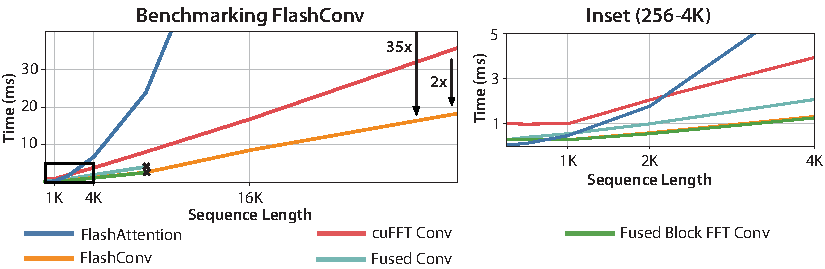
\includegraphics[width=\textwidth]{figs/benchmark_pdf.pdf}
    \caption{\label{fig:fftconv_speed}
      We compare the speed of different algorithms to perform FFT-based
      convolution, along with FlashAttention~\citep{dao2022flashattention} (the fastest attention
      implementation we know of).
      We use batch size 8, hidden dimension 1024, and varying sequence length
      from 256 to 32k, and measure on an A100-SMX4-40GB GPU.
      We see that kernel fusion gives up to 3.4$\times$ speedup over naive FFTConv
      for short sequences (up to 512), block FFT gives up to 2$\times$ speedup for
      medium length sequences (1k - 8k), and state-passing allows 2.3$\times$ faster
      FFTConv for long sequences (16k and above).
    }
\end{figure}
\paragraph{Benchmark \hthree Against Attention}
We benchmark the time to run the forward and backward pass of \hthree with \fastfft against attention.
\fastfft maintains nearly linear scaling, even to very long sequence lengths.
\cref{fig:fftconv_speed} shows overall 2-3$\times$ speedup over FFTConv with cuFFT using our techniques
(block FFT, state-passing).
Simple kernel fusion (even without block FFT) can yield speedup over cuFFT for short sequences, since memory reads/writes are the bottleneck for short sequences.
For long sequences, SSMs using state passing can be dozens of times faster
than even the fastest attention implementation.

%%% Local Variables:
%%% mode: latex
%%% TeX-master: "../main"
%%% End:
